\newpage

\section{Вычислительный эксперимент}

Для анализа моделей, полученных путем дистилляции модели учителя в модель ученика, проводится вычислительный эксперимент для задачи классификации.\\
Эксперимент проводится для выборки FashionMNIST~\cite{FMNIST} - набора изображений предметов одежды. В качестве моделей учителя $\textbf{f}$ и ученика $\textbf{g}$ рассматриваются четырёхслойная и однослойная нейронные сети соответсвенно. Для решения оптимизационной задачи используется Adam, функция активации - ReLu.\\
Выборка разделяется на 3 части: две для обучения многоресурного и малоресурсного доменов, а также тестовая часть выборки. Многоресурсная часть содержит 59000 объектов, малоресурсная часть содержит 1000 объектов, а тестовая часть содержит 10000 объектов.
\newpage
\subsection{Анализ дистилляции Хинтона}

\paragraph{Обучение на обоих доменах.}
Модель учителя и ученика обучаются на обоих доменах.\\
На рис.1а показан график зависимости метрики accuracy на тестовой выборке между истинными метками объектов и вероятностями, предсказанными моделью ученика.\\
На рис.1б показан график зависимости кросс-энтропии на тестовой выборке между истинными метками объектов и вероятностями, предсказанными моделью ученика.\\
На графиках видно, что модель, использующая метки учителя, показывает лучшее значение accuracy, при этом наблюдается значительное снижение ошибки.
\begin{figure}[h!t]\center
\subfloat[]
{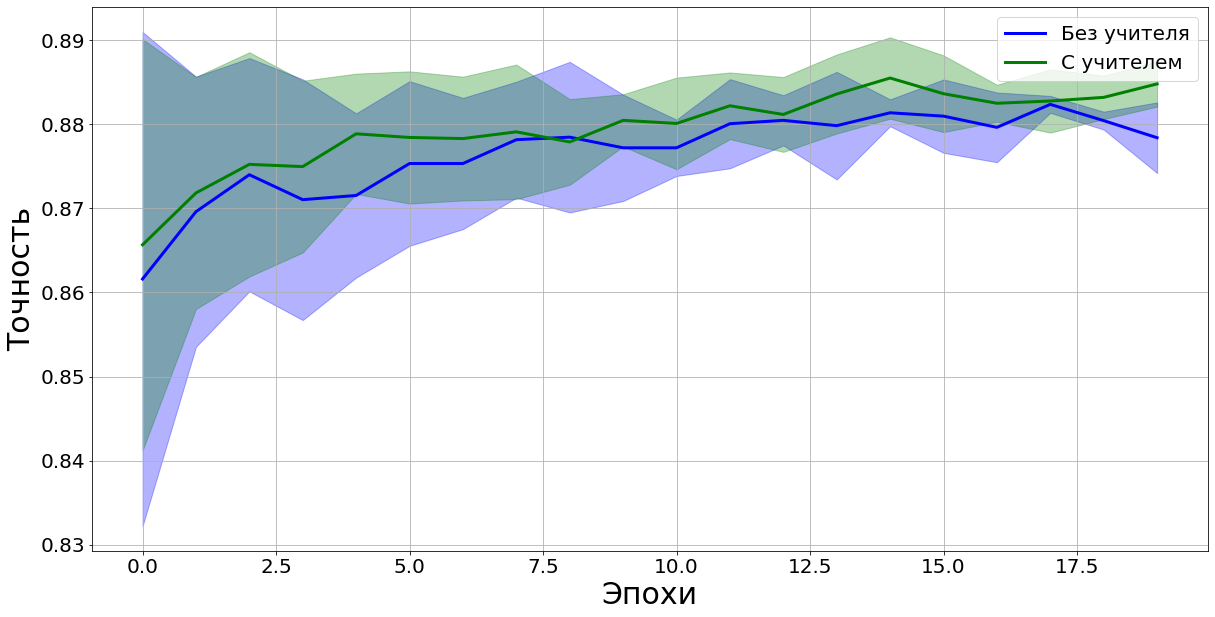
\includegraphics[width=0.5\textwidth]{results/acc}}
\subfloat[]
{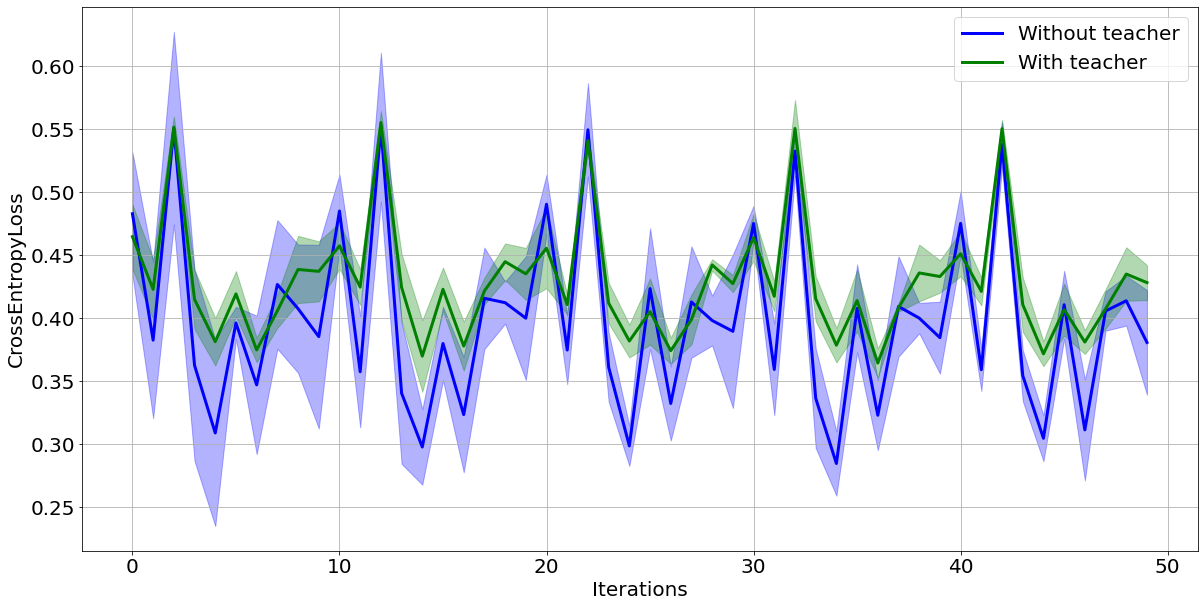
\includegraphics[width=0.5\textwidth]{results/loss}}\\
\caption{Качество аппроксимации на тестовой выборке a) accuracy; b) CrossEntropyLoss между истинными и предсказанными учеником метками}
\end{figure}


\paragraph{Обучение на малоресурсном домене.}
Модель учителя обучается на многоресурсном домене, а модель ученика обучается на малоресурсном домене.\\
На рис.2а показан график зависимости метрики accuracy на тестовой выборке между истинными метками объектов и вероятностями, предсказанными моделью ученика.\\
На рис.2б показан график зависимости кросс-энтропии на тестовой выборке между истинными метками объектов и вероятностями, предсказанными моделью ученика.\\
На графиках видно, что модель, использующая метки учителя, показывает лучшее значение accuracy, при этом наблюдается снижение ошибки.
\begin{figure}[h!t]\center
\subfloat[]
{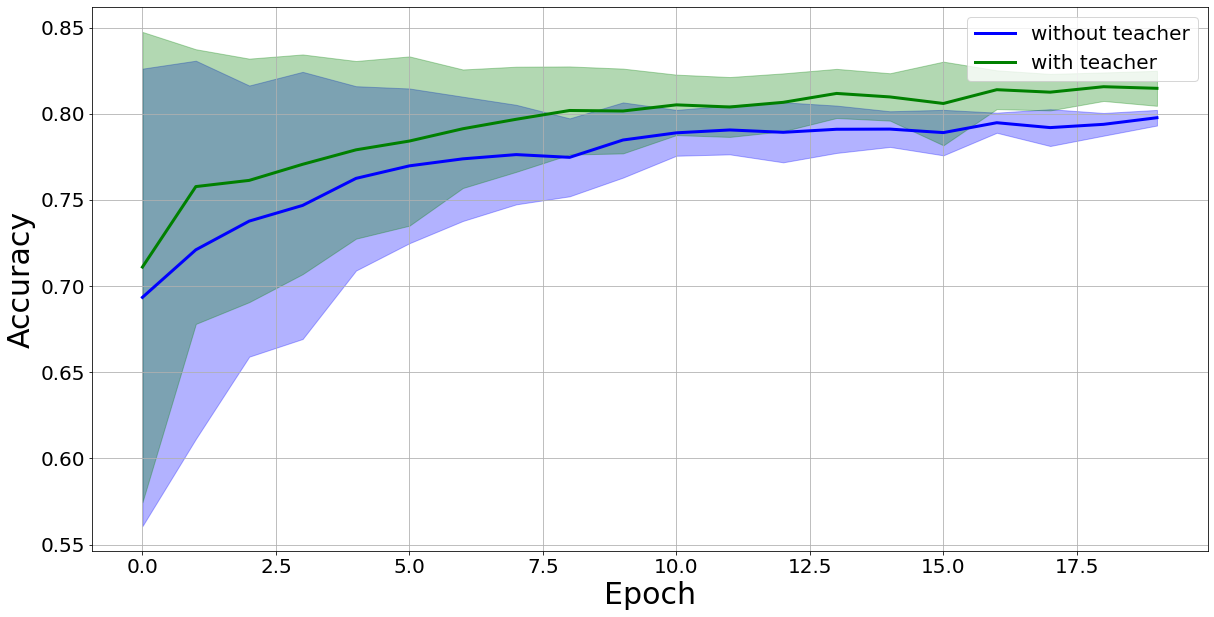
\includegraphics[width=0.5\textwidth]{results/small_acc}}
\subfloat[]
{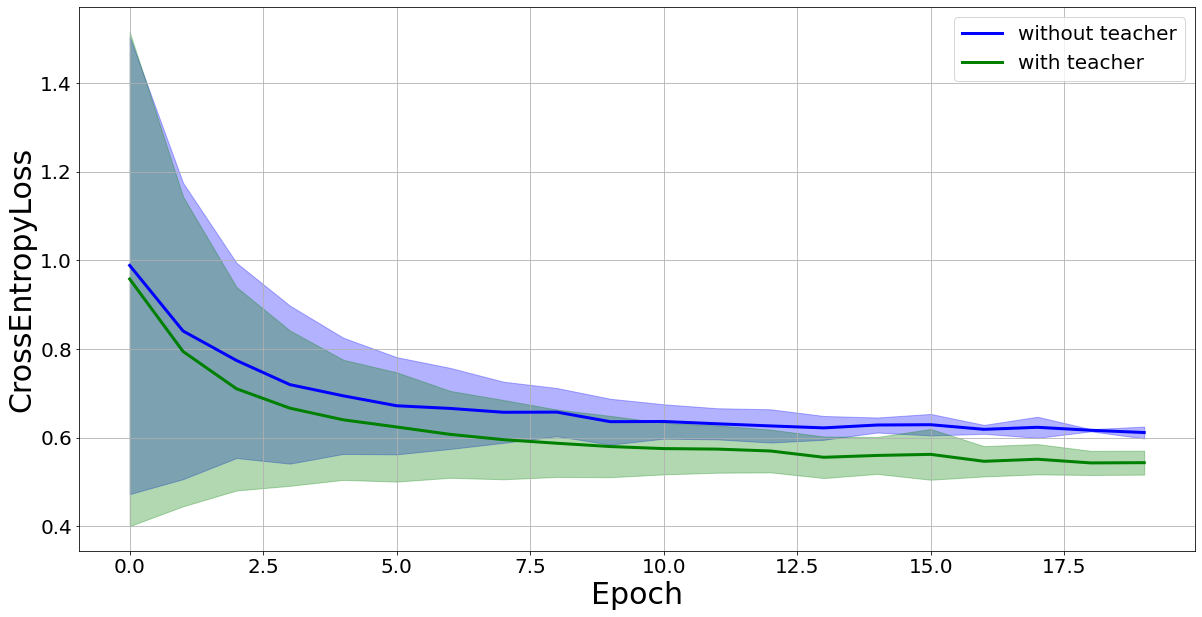
\includegraphics[width=0.5\textwidth]{results/small_loss}}\\
\caption{Качество аппроксимации на тестовой выборке a) accuracy; b) CrossEntropyLoss между истинными и предсказанными учеником метками}
\end{figure}

\paragraph{Обучение на выборке с шумом.}
Добавим к многоресурсному домену нормальный шум $\mathcal{N}(0,0.08)$ и обучим на нем модель учителя. Модель ученика обучается на малоресурсном домене.
\begin{figure}[h!t]\center
{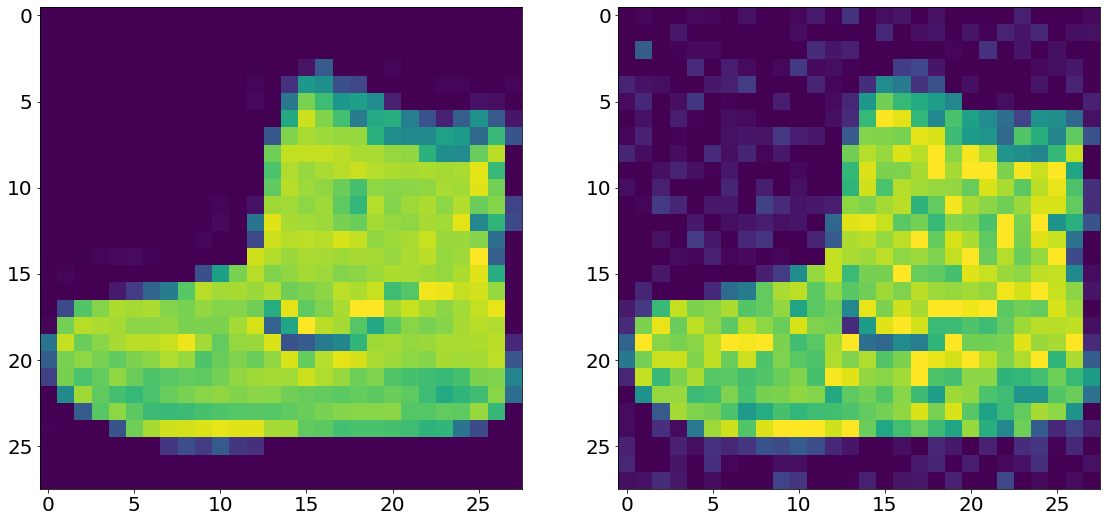
\includegraphics[width=0.5\textwidth]{results/noise}}
\caption{Сравнение объекта выборки до и после добавления шума}
\end{figure}\\
На рис.4а показан график зависимости метрики accuracy на тестовой выборке между истинными метками объектов и вероятностями, предсказанными моделью ученика.\\
На рис.4б показан график зависимости кросс-энтропии на тестовой выборке между истинными метками объектов и вероятностями, предсказанными моделью ученика.\\
На графиках видно, что значения accuracy и CrossEntropyLoss модели, использующей метки учителя на выборке с шумом, лежат между соответствующими значениями для модели без учителя и для модели, использующей метки учителя на выборке без шума.

\begin{figure}[h!t]\center
\subfloat[]
{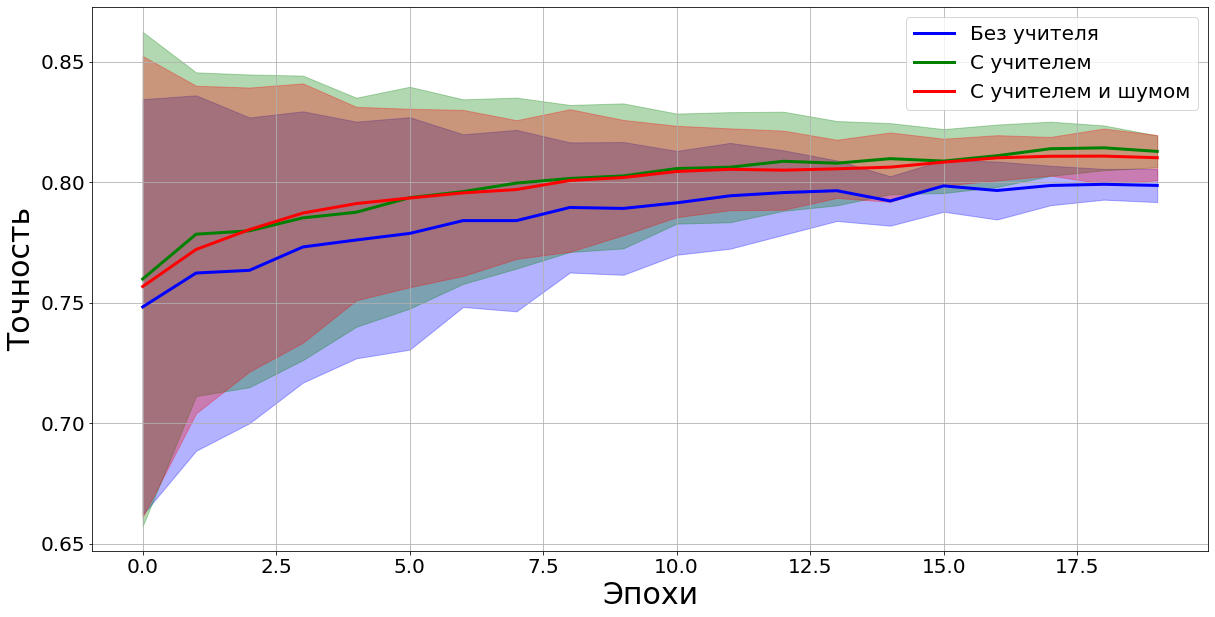
\includegraphics[width=0.5\textwidth]{results/noise_acc}}
\subfloat[]
{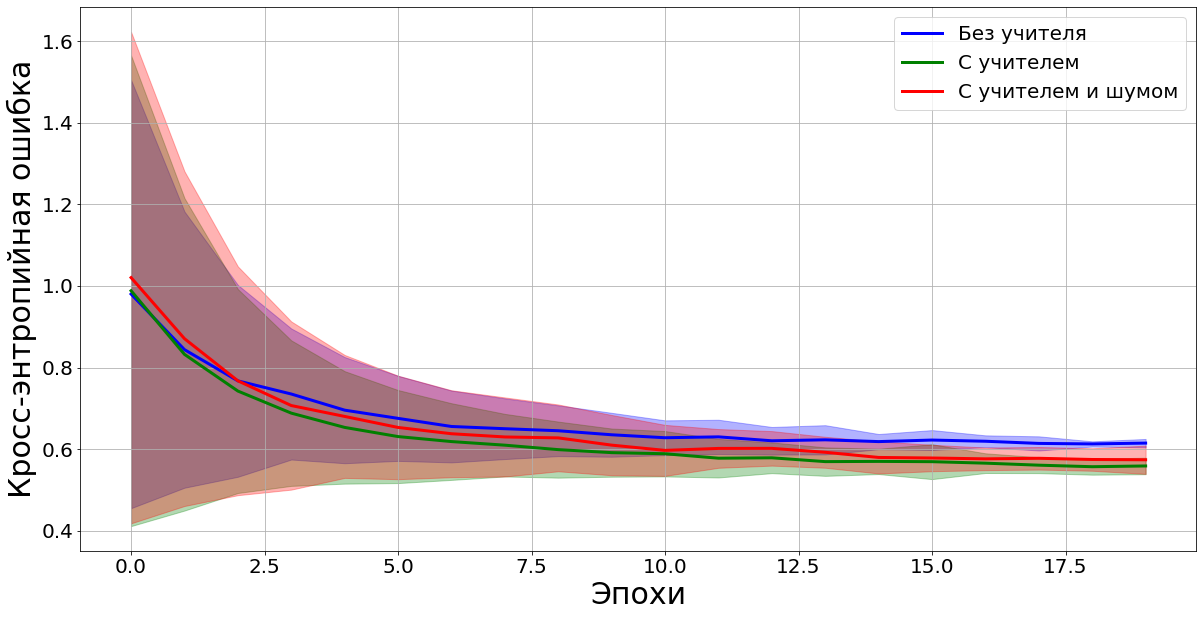
\includegraphics[width=0.5\textwidth]{results/noise_loss}}\\
\caption{Качество аппроксимации на тестовой выборке a) accuracy; b) CrossEntropyLoss между истинными и предсказанными учеником метками}
\end{figure}

\paragraph{Обучение на выборке с dilation.}
Применим к многоресурсному домену сверточное преобразование с параметром $\text{dilation}=2$ и обучим на нем модель учителя. Модель ученика обучается на малоресурсном домене.\\
\begin{figure}[h!t]\center
{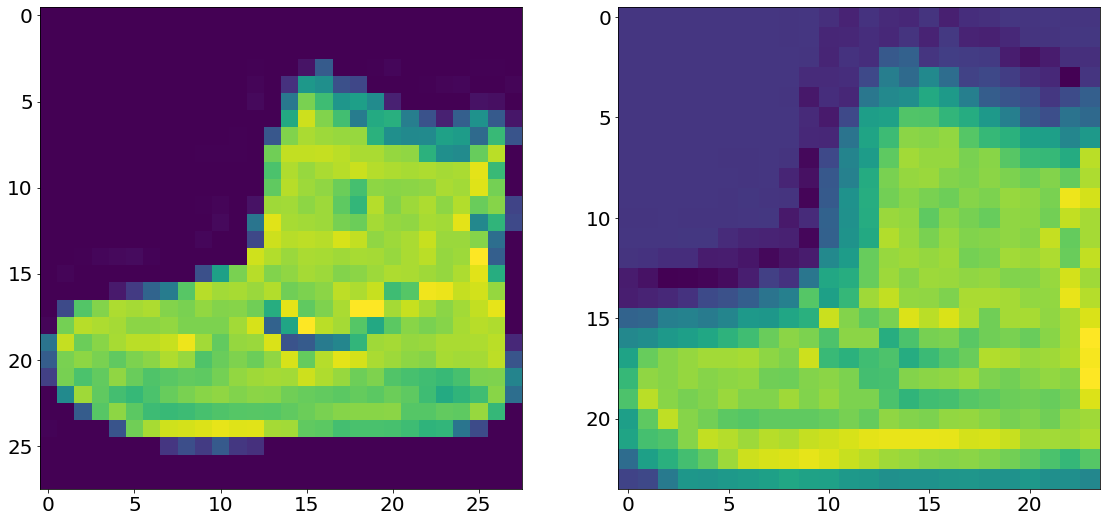
\includegraphics[width=0.5\textwidth]{results/dilation}}
\caption{Сравнение объекта выборки до и после преобразования}
\end{figure}\\
На рис.6а показан график зависимости метрики accuracy на тестовой выборке между истинными метками объектов и вероятностями, предсказанными моделью ученика.\\
На рис.6б показан график зависимости кросс-энтропии на тестовой выборке между истинными метками объектов и вероятностями, предсказанными моделью ученика.\\
На графиках видно, что значения accuracy и CrossEntropyLoss модели, использующей метки учителя на выборке с преобразованием, лежат между соответствующими значениями для модели без учителя и для модели, использующей метки учителя на выборке без преобразования.
\begin{figure}[h!t]\center
\subfloat[]
{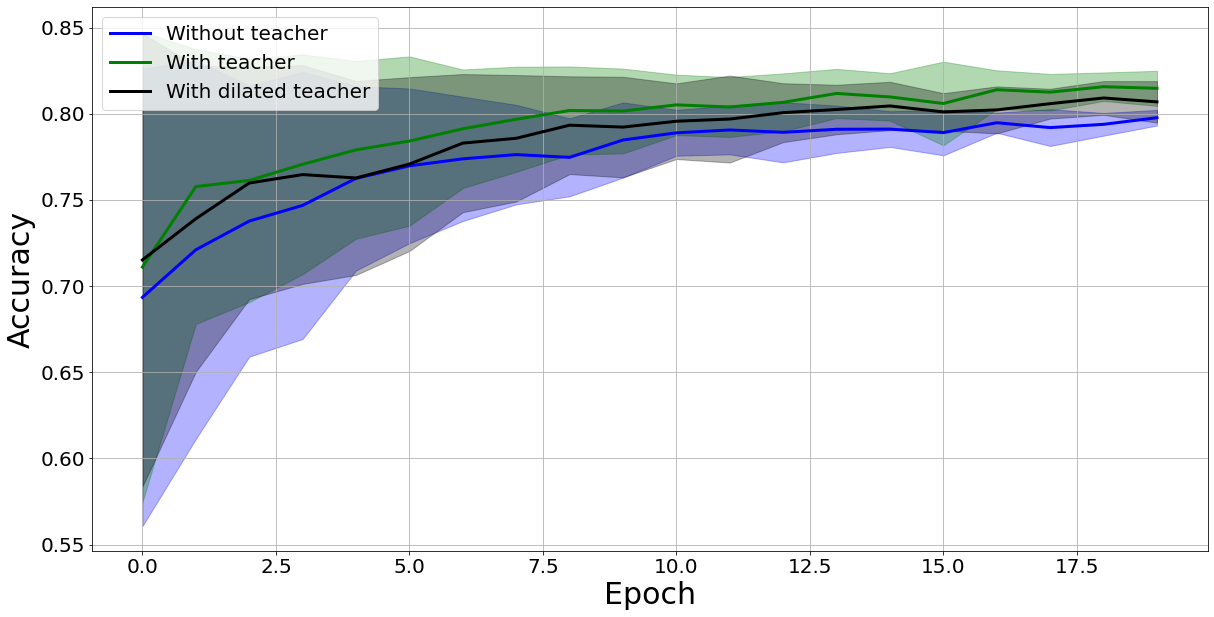
\includegraphics[width=0.5\textwidth]{results/dilation_acc}}
\subfloat[]
{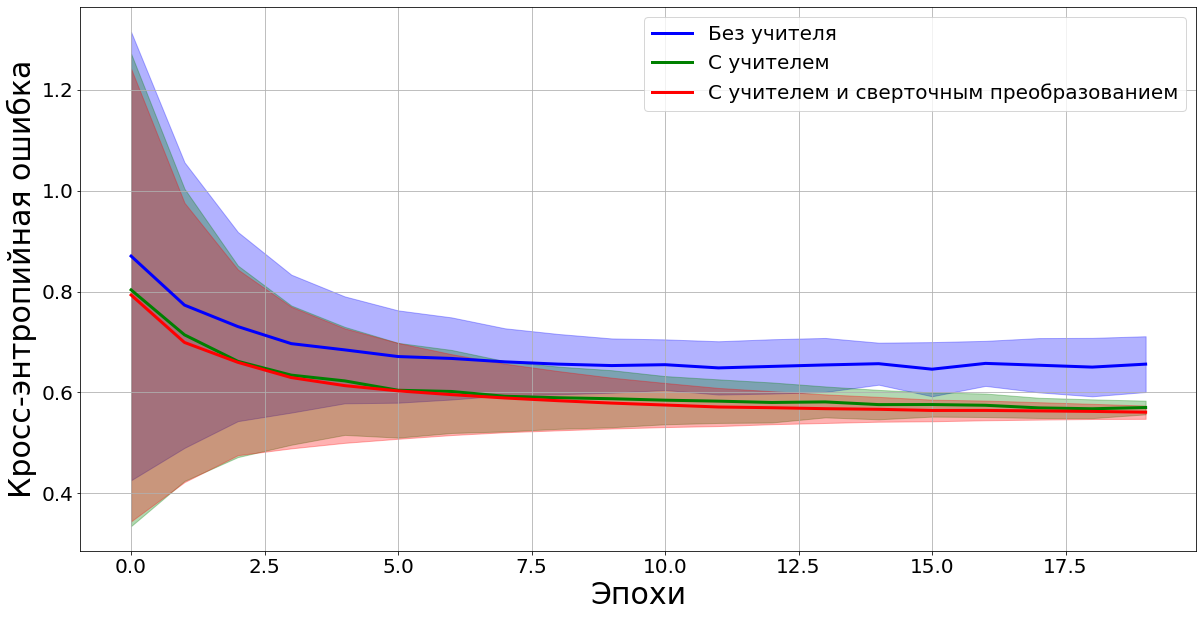
\includegraphics[width=0.5\textwidth]{results/dilation_loss}}\\
\caption{Качество аппроксимации на тестовой выборке a) accuracy; b) CrossEntropyLoss между истинными и предсказанными учеником метками}
\end{figure}

